\documentclass[12pt]{article}
\usepackage[a4paper, total={7.5in, 10in}]{geometry}
\usepackage{array}
\usepackage{graphicx, subfig, wrapfig, fancyhdr, lastpage, multicol ,color,arydshln,makecell, chemfig}

\newcommand\headerMe[2]{\noindent{}#1\hfill#2}
\usepackage[mathscr]{euscript}
\usepackage{tabularray}

\setlength{\columnseprule}{1pt}
\def\columnseprulecolor{\color{blue}}


\pagestyle{fancy}
\fancyhf{}

\cfoot{ \em{Page \thepage \hspace{1pt} / \pageref{LastPage}}}
\begin{document}

\headerMe{Royaume du Maroc}{année scolaire \emph{2023-2024}}\\
\headerMe{Ministère de l'Éducation nationale, }{  Professeur :\emph{Zakaria Haouzan}}\\
\headerMe{du Préscolaire et des Sports}{Établissement : \emph{Lycée SKHOR qualifiant}}\\
%\vspace{-1cm}
\begin{center}
Devoir Surveillé  N°2 - S2 \\
    2ème année baccalauréat Sciences physiques\\
Durée 2h00
\\
    \vspace{.2cm}
\hrulefill
\Large{Chimie 7pts - 45min}
\hrulefill\\

    \emph{Les deux parties sont indépendantes}
\end{center}
%end Headerss------------------------
%__________________Chimie ______________________-
%%%%%%%+_+_+_+_+_+_+_+_+_Partie1

 \section*{Partie I-Etude de la pile argent-chrome}
\begin{wrapfigure}[3]{r}{0.4\textwidth}
	\vspace{-2.5cm}
\begin{center}
  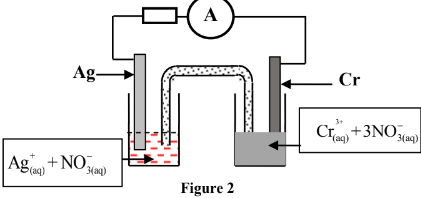
\includegraphics[width=0.4\textwidth]{./img/pileex_5.png}
\end{center}
\end{wrapfigure}

Cette partie se propose d’étudier une pile électrochimique.
Cette pile est constituée :

- d’une électrode en chrome (Cr) plongée dans
une solution aqueuse de nitrate de chrome (III) $(Cr^{3+}_{(aq)} + 3NO^-_{(aq)})$

- d’une électrode en argent (Ag) plongée dans
une solution aqueuse de nitrate d’argent $(Ag^+_{(aq)} + NO^-_{(aq)}) $

- d’un pont salin qui relie les deux solutions.
On branche un conducteur ohmique en série avec
un ampèremètre, et on place le dipôle, ainsi constitué, entre les pôles de la pile (figure 2).
L’ampèremètre indique le passage d’un courant électrique, d’intensité constante, dans le circuit.
Après une durée $(\Delta{t})$
de fonctionnement de la pile, on observe un dépôt sur l’électrode d’argent et une
diminution de la masse de l’électrode de chrome.

\textbf{\underline{Données:}}
\begin{itemize}
  \item La constante de Faraday : $F=9,65.10^{4} C.mol^{-1} $;
  \item Masse molaire du chrome : $M(Cr) = 52 g/mol $.
\end{itemize}

\begin{enumerate}
  \item Préciser l’anode de la pile. Justifier\dots(0,75pt)
  \item Représenter le schéma conventionnel de la pile\dots(0,75pt)
  \item Ecrire les équations aux électrodes ainsi que l’équation bilan lors du fonctionnement de la pile\dots(1pt)
  \item Sachant que la quantité d'électricité débitée par la pile pendant la durée $\Delta{t}$ est : $Q=5,79C$,déterminer la variation $\Delta{m}$ de la masse de l’électrode de chrome\dots(1pt)
\end{enumerate}


 \section*{Partie II- Etude de la pile nickel-cadmium.}

\emph{Lors de leur fonctionnement, les piles électrochimiques convertissent une partie de l’énergie
chimique en énergie électrique. On étudie dans cette partie de l’exercice le principe de
fonctionnement de la pile nickel-cadmium.}

On réalise la pile nickel-cadmium en utilisant le matériel et les produits suivants :

\begin{itemize}
  \item un bécher contenant une solution aqueuse de sulfate de nickel $Ni^{2+}_{(aq)} + SO^{2-}_{4(aq)}$ de concentration
molaire $C_1 =1 mol/L$

\item un bécher contenant une solution aqueuse de sulfate de cadmium $Cd^{2+}_{(aq)} + SO^{2-}_{4(aq)}$ de concentration
molaire $C_2 = 1mol/L$
\item une lame de nickel et une lame de cadmium.
\item un pont salin.
\end{itemize}

On relie les électrodes de la pile à un conducteur ohmique en série avec un ampèremètre qui
indique le passage d’un courant électrique d’intensité constante $I_A = 0,3$ dans le circuit.

\textbf{\underline{Données:}}
\begin{itemize}
  \item La constante de Faraday : $F=9,65.10^{4} C.mol^{-1} $.
  \item La masse molaire du cuivre: $M(Ni) = 58,7 g/mol$.
  \item La constante d'équilibre associée à l'équation $Ni^{2+}_{(aq)} + Cd_{(s)} \rightleftharpoons	
 Cd^{2+}_{(aq)} + Ni_{(s)} $ est $K =4,5.10^{5}$.
\end{itemize}


\begin{enumerate}
  \item Calculer la valeur du quotient de réaction $Q_{r,i}$ à l’état initial du système chimique.\dots(0,5pt)
  \item  En déduire le sens d'évolution spontanée du système chimique et Donner le schéma conventionnel de cette pile.\dots(1pt)
  \item Ecrire l’équation de la réaction chimique à chaque la cathode.\dots(1pt)
  \item La pile fonctionne pendant une durée $\Delta{t} = 5h$ . Calculer la masse $m(Ni)$ Cu du cuivre déposé
    pendant la durée $\Delta{t}$.\dots(1pt)
\end{enumerate}

%\hrulefill
%\Large{Physique 13pts/78min}
%\hrulefill\\
%\newpage
\begin{center}
    %\vspace{.60cm}
\hrulefill
\Large{Physique 13pts - 75min}
\hrulefill\\
    \emph{Les parties sont indépendantes}
\end{center}

%\vspace{-1cm}
\section*{Partie I : Mouvement d’un solide dans le champ de pesanteur}

\emph{L’étude des mouvements des solides dans le champ de pesanteur uniforme permet de déterminer les
grandeurs caractéristiques de ces mouvements.
L’objectif de cette partie de l’exercice est d’étudier le mouvement d’une balle dans le champ de
pesanteur uniforme.}


\begin{center}
  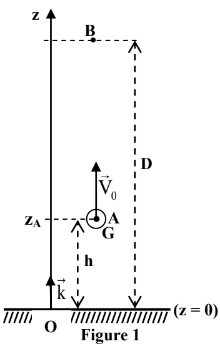
\includegraphics[width=0.22\textwidth]{./img/chute_verticale.png}
  \hspace{2cm}
  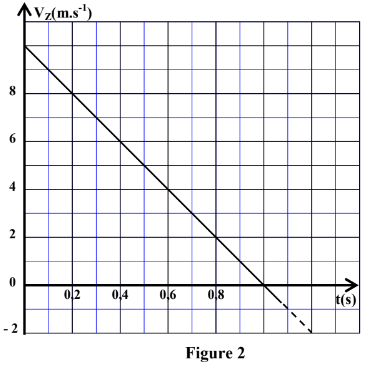
\includegraphics[width=0.4\textwidth]{./img/chute_ve_courbe.png}
\end{center}



On lance verticalement vers le haut avec une vitesse initiale
$\vec{V_0}$, à un instant choisi comme origine des dates $(t=0)$ , une balle de masse m d’un
point A situé à une hauteur $h = 1,2 m$ du sol.

On étudie le mouvement du centre d’inertie G de la balle dans un
référentiel terrestre considéré galiléen. On repère la position de G,
à un instant t, dans le repère $(O, \vec{k})$ par la cote z ( Figure 1).
On considère que les forces de frottement et la poussée d’Archimède sont
négligeables.

\textbf{Données : }L’intensité de la pesanteur $g = 10 m/s^2$

\begin{enumerate}
  \item Définir la chute libre\dots(1pt)

  \item En appliquant la deuxième loi de Newton, établir l’équation
    différentielle vérifiée par la vitesse Vz du centre d’inertie $G$ \dots(1pt)

  \item Monter que l’équation horaire du mouvement de G s’écrit\dots(1pt) $$z = -\frac{1}{2}.g.t^2 + V_0.t + h$$

  \item La courbe de la figure 2 représente les variations de
la vitesse $V_z$ en fonction du temps.
En exploitant le graphe de la figure 2, écrire
    l’expression numérique de la vitesse $V_z = f(t)$\dots(0,75pt)
  
  \item Le centre d’inertie G passe, au cours de la montée,
    par le point B situé à une hauteur $D$ du sol, avec une vitesse $V_B = 3m/s$ (figure1). Montrer que $D=5,75m$\dots(1pt)

\item On lance de nouveau, à un instant choisi comme
nouvelle origine des dates $(t=0)$ , verticalement vers le
haut, la balle du même point A avec une vitesse
initiale $V'_0 =8m/s$. Le centre d’inertie G de la balle
    atteint-il le point B? Justifier votre réponse\dots(1pt)

\end{enumerate}

\section*{Partie II : Le ski sur la glace}
Le but de cet exercice est d’étudier le mouvement d’un sportif, pratiquant le ski sur
des trajectoires de glace diverses.
Le circuit de ski représenté sur la figure ci-dessous, est constitué de trois parties :


\begin{center}
  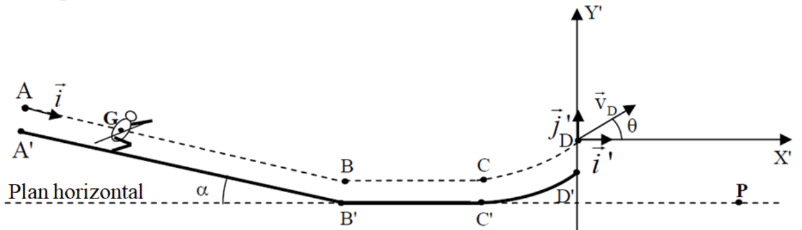
\includegraphics[width=0.9\textwidth]{./img/mvt_plan.png}
\end{center}

- Une partie A’B’ rectiligne de longueur A’B’ = 82,7 m, inclinée d’un angle $\alpha = 14^{\circ}$
par rapport au plan horizontal.

- Une partie B’C’ rectiligne horizontale, de longueur L = 100 m.

- Une partie C’D’ circulaire.

On modélise le sportif et ses accessoires par un solide (S) de masse $m = 65 Kg$, et de
centre d’inertie G. On prendra : $g = 10 m.s^{-2}$

G passe au cours de son mouvement par les positions A, B, C et D représentées sur la
figure, tel que : A’B’ = AB et B’C’ = BC.

\textbf{1 - Etude du mouvement sur la partie A’B’ :}

A l’instant t = 0, G part de A sans vitesse initiale, le solide (S) glisse ainsi sans
frottements sur la partie A’B’.

On repère la position de G, à un instant t, par l’abscisse x dans le repère $(A.\vec{i})$ , et on considère que xG = 0 à l’instant t = 0.


\begin{enumerate}
  \item[1.1.] Par application de la deuxième loi de Newton, établir l’expression de
l’accélération aG du mouvement de G en fonction de $g$ et $\alpha$.\dots(1pt)
\item[1.2.] Déterminer en justifiant votre réponse la nature du mouvement de G sur
  cette partie\dots(1pt)
\item[1.3.] A l’aide des équations horaires du mouvement, trouver la valeur $v_B$ de la
vitesse de G lors du passage par la position B\dots(1pt)
  \end{enumerate}

  \textbf{2- Etude du mouvement sur la partie B’C’ :}
  
  Le solide (S) poursuit son mouvement sur la partie B’C’, où il subit des frottements
modélisées par une force $\vec{f}$ constante, tangente à la trajectoire et de sens inverse à
celui du mouvement.

On considère que la valeur de la vitesse de G au point B ne varie pas lors du passage
du solide (S) du plan incliné au plan horizontal.
Pour étudier le mouvement de G sur cette partie, on choisit, un repère horizontal
d’origine confondue avec le point B, et l’instant du passage de G en ce point comme
nouvelle origine des temps

\begin{enumerate}
  \item[2.1.] En appliquant la deuxième loi de Newton, déterminer la nature du
    mouvement de G sur le trajet BC\dots(1pt)
\item[2.2.] Trouver l’expression de l’intensité f de la force de frottement en fonction
  de m, L, $v_B$ et $v_C$ vitesse de G au point C, puis calculer f\dots(1pt)
  \end{enumerate}
On donne : $v_C = 12 m.s^{-1}$.

\textbf{3- Etude du mouvement dans le champ de pesanteur uniforme :}

Lorsque le solide (S) quitte la piste, G passe en D, à un instant considéré comme
nouvelle origine des temps, avec une vitesse $v_D$ inclinée d’un angle $\theta = 45^{\circ}$ par

rapport au plan horizontal. Le solide (S) tombe à la position P.
On étudie le mouvement de G dans le repère galiléen

$(D,\vec{i'}, \vec{j'})$ , et on néglige l’action
de l'air au cours du mouvement.

\begin{enumerate}
  \item[3.1.] Trouver les expressions littérales des équations horaires $x(t)$ et $y(t)$ du
mouvement de G, et déduire l’expression littérale de l’équation de la
    trajectoire\dots(1,25pt)
  \item[3.2.] Déterminer $v_D$, la vitesse de G au moment où il quitte le point D, sachant
    que les coordonnées de G à l’arrivée en P sont : $x_G = 15 m$ et $y_G = - 5 m$\dots(1pt)
  \end{enumerate}

%\begin{wrapfigure}[9]{r}{0.25\textwidth}
  %\begin{center}
	  %\vspace{-1cm}
	%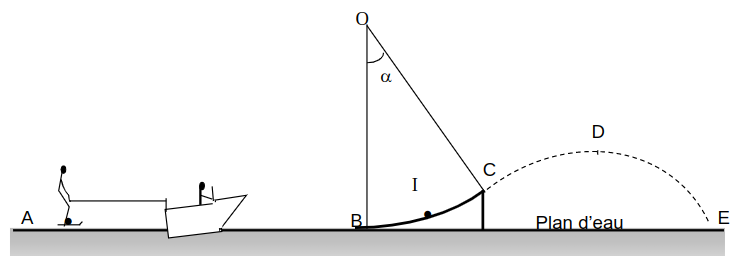
\includegraphics[width=0.19\textwidth]{./img/img01.png}
	%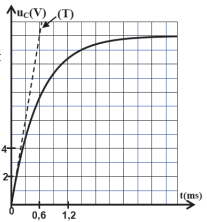
\includegraphics[width=0.25\textwidth]{./img/img02.png}
  %\end{center}
%\end{wrapfigure}

   % \begin{wrapfigure}[7]{r}{0.32\textwidth}
  %\begin{center}

	  %\vspace{-1.6cm}
	%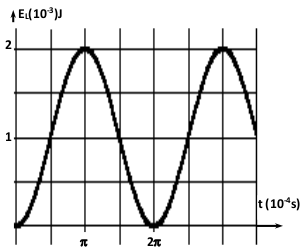
\includegraphics[width=0.32\textwidth]{./img/ex_02.png}
  %\end{center}
%\end{wrapfigure}



\end{document}
